\chapter{Simple Linear Regression}
\label{chap:simple_linear_regression}

% ========================================
% SECTION 1: INTRODUCTION
% ========================================
\section{Introduction: What is Regression?}
Imagine you are a college student appearing for campus placements. You notice a pattern among your seniors: those with higher CGPAs tend to get higher salary packages.

\begin{itemize}
    \item \textbf{Student A}: 6.0 CGPA $\rightarrow$ 4 LPA
    \item \textbf{Student B}: 7.0 CGPA $\rightarrow$ 6 LPA
    \item \textbf{Student C}: 9.0 CGPA $\rightarrow$ ?
\end{itemize}

Your intuition tells you that Student C will likely get something higher than 6 LPA, perhaps around 10 LPA. What your brain just did is called \textbf{Regression}. You identified a relationship between an input (CGPA) and an output (Package) and used it to predict a future value.

\begin{definition}
\textbf{Regression}: A supervised learning technique where the goal is to predict a \textbf{continuous} numerical output variable based on one or more input features.
\end{definition}

\begin{definition}
\textbf{Linear Regression}: A specific type of regression where we assume the relationship between the input ($x$) and output ($y$) can be represented by a \textbf{straight line}.
\end{definition}

% ========================================
% SECTION 2: INTUITION
% ========================================
\section{Intuition: The Line of Best Fit}
Let us visualize this concept. Suppose we plot each student as a point on a graph, with CGPA on the X-axis and Package on the Y-axis.

\begin{figure}[htbp]
\centering
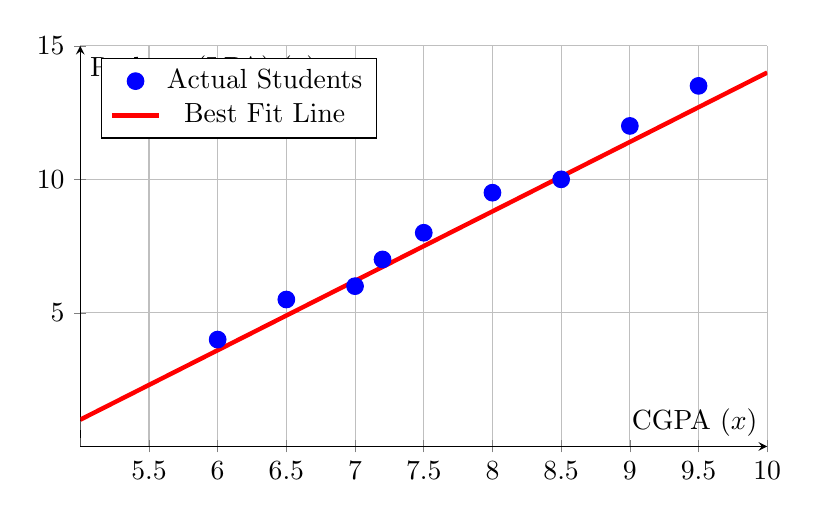
\begin{tikzpicture}
    \begin{axis}[
        xlabel={CGPA ($x$)},
        ylabel={Package (LPA) ($y$)},
        xmin=5, xmax=10,
        ymin=0, ymax=15,
        axis lines=middle,
        grid=major,
        width=0.85\textwidth,
        height=0.55\textwidth,
        legend pos=north west
    ]
    % Data Points
    \addplot[only marks, mark=*, color=blue, mark size=3pt] coordinates {
        (6, 4) (6.5, 5.5) (7, 6) (7.2, 7) (7.5, 8) (8, 9.5) (8.5, 10) (9, 12) (9.5, 13.5)
    };
    \addlegendentry{Actual Students}
    
    % Regression Line
    \addplot[domain=5:10, color=red, ultra thick] {2.6*x - 12};
    \addlegendentry{Best Fit Line}
    
    % Intercept Annotation
    \draw[dashed, gray] (axis cs:5, 0) -- (axis cs:5, 1);
    \node[left] at (axis cs:5, 1) {$c$ (Intercept)};
    \end{axis}
\end{tikzpicture}
\caption{The ``Best Fit Line'' passes through the center of the scattered data points.}
\label{fig:best_fit_intuition}
\end{figure}

The goal of Linear Regression is to find the \textbf{Best Fit Line}. Imagine holding a stick over the scatter plot:
\begin{enumerate}
    \item You move the stick up, down, and rotate it.
    \item Your goal is to make the stick pass \textit{as close as possible} to all the points.
    \item Mathematically, you are minimizing the total ``distance'' (error) between the points and your stick.
\end{enumerate}

% ========================================
% SECTION 3: MATHEMATICAL FORMULATION
% ========================================
\section{Mathematical Formulation}
Every straight line in the world can be written as:
\begin{equation}
    y = mx + c
    \label{eq:line}
\end{equation}
In Machine Learning, we often use slightly different notation ($\beta$ for coefficients):
\begin{equation}
    y = \beta_0 + \beta_1 x
\end{equation}

\begin{itemize}
    \item $y$: The \textbf{Target} (Dependent Variable). This is what we want to predict (e.g., Package).
    \item $x$: The \textbf{Feature} (Independent Variable). This is our input (e.g., CGPA).
    \item $\beta_1$ (or $m$): The \textbf{Slope} or \textbf{Weight}. It tells us how steeply the Package rises with CGPA. A high slope means a small increase in CGPA leads to a huge jump in salary.
    \item $\beta_0$ (or $c$): The \textbf{Intercept} or \textbf{Bias}. This is the baseline value. If CGPA were 0, this would be the predicted package. (Mathematically necessary, though practically, no one has 0 CGPA.)
\end{itemize}

\textbf{The Core Question}: How do we find the optimal values of $m$ and $c$?

% ========================================
% SECTION 4: WORKED EXAMPLE (OLS DERIVATION)
% ========================================
\section{Finding $m$ and $c$: Ordinary Least Squares (OLS)}
This is the heart of Linear Regression. We will derive the formulas step-by-step.

\subsection{Step 1: Define the Error}
For any single data point $i$, the \textbf{error} (or \textbf{residual}) is the difference between the actual value ($y_i$) and the predicted value ($\hat{y}_i$).
\begin{equation}
    \text{Residual}_i = y_i - \hat{y}_i = y_i - (mx_i + c)
\end{equation}

\subsection{Step 2: Define the Loss Function (SSE)}
We cannot simply add up the errors because positive and negative errors cancel each other out.
\textbf{Solution}: Square the errors. This removes negative signs and penalizes large errors more heavily.
\begin{definition}
\textbf{Sum of Squared Errors (SSE)}: The total squared difference between actual and predicted values.
\begin{equation}
    J(m, c) = \sum_{i=1}^{n} (y_i - \hat{y}_i)^2 = \sum_{i=1}^{n} (y_i - mx_i - c)^2
\end{equation}
\end{definition}
\textbf{Goal}: We want to find the values of $m$ and $c$ that \textbf{minimize} $J$.

\subsection{Step 3: Minimize Loss using Calculus}
To find the minimum of a curve, we take the derivative and set it to zero.

\textbf{(A) Derivative with respect to $c$:}
\begin{align}
    \frac{\partial J}{\partial c} &= \sum 2(y_i - mx_i - c)(-1) = 0 \\
    -2 \sum (y_i - mx_i - c) &= 0 \\
    \sum y_i - m \sum x_i - nc &= 0 \\
    c &= \bar{y} - m\bar{x}
\end{align}
Where $\bar{y} = \frac{\sum y_i}{n}$ and $\bar{x} = \frac{\sum x_i}{n}$ are the means.

\textbf{(B) Derivative with respect to $m$:}
After substituting $c$ and simplifying (algebra omitted for brevity), we get:
\begin{equation}
    \boxed{m = \frac{\sum (x_i - \bar{x})(y_i - \bar{y})}{\sum (x_i - \bar{x})^2}}
    \label{eq:ols_m}
\end{equation}
\begin{equation}
    \boxed{c = \bar{y} - m\bar{x}}
    \label{eq:ols_c}
\end{equation}
These are the famous \textbf{OLS formulas}.

% ========================================
% SECTION 5: CODE IMPLEMENTATION
% ========================================
\section{Implementation in Python}
Let us build a Simple Linear Regression model using \texttt{scikit-learn}.

\begin{lstlisting}[language=Python, caption=Simple Linear Regression with Scikit-Learn]
import numpy as np
import matplotlib.pyplot as plt
from sklearn.linear_model import LinearRegression

# =============================================
# STEP 1: Create Dummy Data
# =============================================
np.random.seed(42)  # For reproducibility
# 100 students with CGPA between 5 and 10
X = np.random.uniform(5, 10, 100).reshape(-1, 1)
# Package roughly follows: 2.5 * CGPA - 8 (plus noise)
y = 2.5 * X - 8 + np.random.normal(0, 1.5, (100, 1))

# =============================================
# STEP 2: Train the Model
# =============================================
model = LinearRegression()
model.fit(X, y)  # The model calculates 'm' and 'c' using OLS

# =============================================
# STEP 3: Check Learned Parameters
# =============================================
print(f"Slope (m): {model.coef_[0][0]:.4f}")       # Expected: ~2.5
print(f"Intercept (c): {model.intercept_[0]:.4f}") # Expected: ~-8

# =============================================
# STEP 4: Visualize the Result
# =============================================
plt.figure(figsize=(10, 6))
plt.scatter(X, y, color='blue', alpha=0.6, label='Actual Data')
plt.plot(X, model.predict(X), color='red', linewidth=2, label='Best Fit Line')
plt.xlabel('CGPA')
plt.ylabel('Package (LPA)')
plt.title('Simple Linear Regression')
plt.legend()
plt.grid(True)
plt.show()
\end{lstlisting}

% ========================================
% SECTION 6: VISUALIZATION (Already in Section 2)
% ========================================
% (Visualization is integrated into Section 2 with TikZ)

% ========================================
% SECTION 7: SUMMARY / KEY TAKEAWAYS
% ========================================
\section{Key Takeaways}
\begin{enumerate}
    \item \textbf{Assumption}: Linear Regression assumes the data follows a straight line ($y = mx + c$).
    \item \textbf{Goal}: Find the line that minimizes the Sum of Squared Errors (SSE).
    \item \textbf{Parameters}: The model learns two things:
    \begin{itemize}
        \item \textbf{Slope ($m$)}: The strength of the relationship.
        \item \textbf{Intercept ($c$)}: The baseline value.
    \end{itemize}
    \item \textbf{Method}: Ordinary Least Squares (OLS) provides a closed-form formula for $m$ and $c$.
\end{enumerate}

% ========================================
% SECTION 8: HOTS QUESTIONS
% ========================================
\section{HOTS: Interview Questions}
\textbf{Q1: What are the key assumptions of Linear Regression?}
\begin{itemize}
    \item \textbf{Linearity}: The relationship between $X$ and $Y$ is linear.
    \item \textbf{Independence}: Observations are independent.
    \item \textbf{Homoscedasticity}: Constant variance of errors.
    \item \textbf{Normality}: Residuals should be normally distributed.
    \item \textbf{No Multicollinearity}: Features should not be highly correlated with each other.
\end{itemize}

\textbf{Q2: Why do we square the residuals instead of using absolute values?}
\begin{itemize}
    \item Squaring removes negative signs, ensuring errors do not cancel out.
    \item Squaring penalizes larger errors more heavily.
    \item The squared function is \textbf{smooth} (differentiable everywhere), which is essential for optimization algorithms like Gradient Descent.
    \item The absolute value function $|x|$ has a sharp ``V'' shape at zero, making it non-differentiable at that point.
\end{itemize}

\textbf{Q3: Is OLS suitable for very large datasets?}
\begin{itemize}
    \item Not always. OLS involves matrix inversion ($(X^TX)^{-1}$), which has a time complexity of $O(n^3)$.
    \item For massive datasets, \textbf{Gradient Descent} is preferred as it iteratively approximates the solution with lower memory usage.
\end{itemize}
